\chapter{\uppercase{Taules}}
\section{Títol de la secció}
\paragraph{Anem a inserir una figura amb i es pot afegir una etiqueta i un peu de figura. La seva referència: \ref{fig:x cubed graph}.}
%\verb|\label{fig:x cubed graph}]{nom}|
%\verb|\includegraphics[scale=0.5]{nom}|
% \verb|\begin{figure}|,
% \verb|\end{figure}|,
%\verb|\label{fig:x cubed graph}|
\begin{figure}[H]
\centering
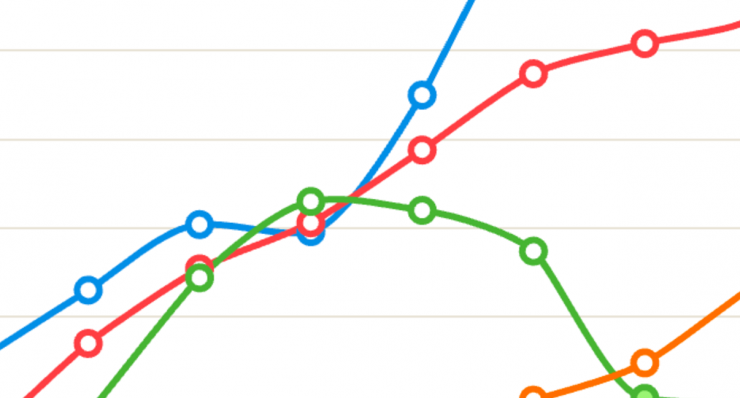
\includegraphics[scale=0.5]{graph_a}
\caption{Figura}
\label{fig:x cubed graph}
\end{figure}
fs
fs
%
%https://ercanozturk.org/2017/12/16/python-matplotlib-plots-in-latex/
%
\subsection{Títol de la subsecció}
Escriure \verb|[h!]| per forçar la imatge a la posició que toca, sinó pot saltar de pàgina per optimitzar espai. Podria ser més estricte amb The float package.
%(\usepackage{float}) allows to set the option to [H], which is even stricter than [h!].\\
\begin{figure}[h!]
	\centering
	\begin{subfigure}[b]{0.3\textwidth}
	\centering
	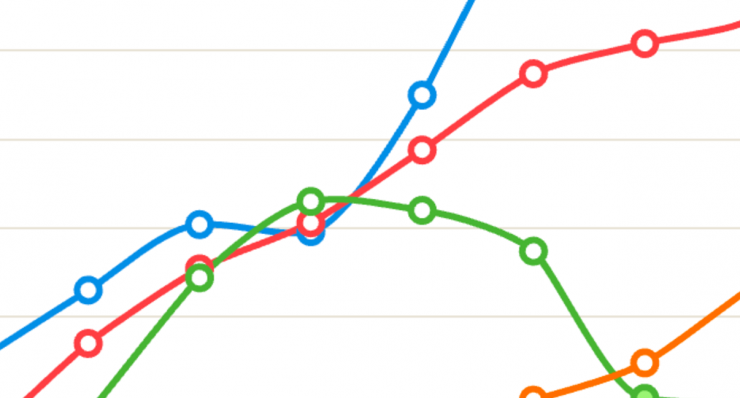
\includegraphics[width=\textwidth]{graph_a}
	\caption{$y=x$}
	\label{fig: y equals x}
	\end{subfigure}
	\hfill
	%afegir una línia en blanc fa salt de línia
	\begin{subfigure}[b]{0.3\textwidth}
	\centering
	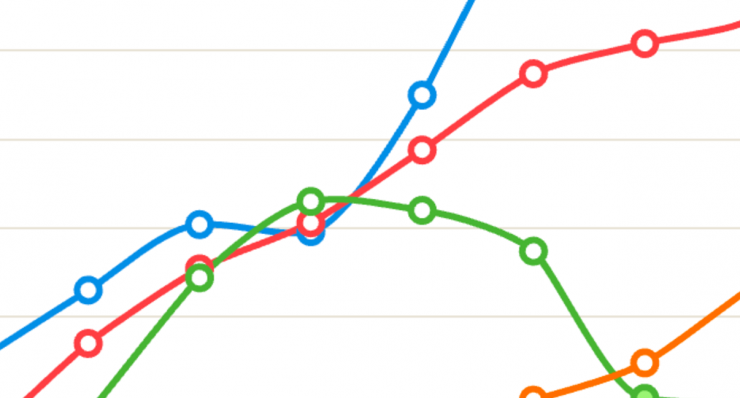
\includegraphics[width=\textwidth]{graph_a}
	\caption{$y=x$}
	\label{fig: y equals x}
	\end{subfigure}
	\hfill
	\begin{subfigure}[b]{0.3\textwidth}
	\centering
	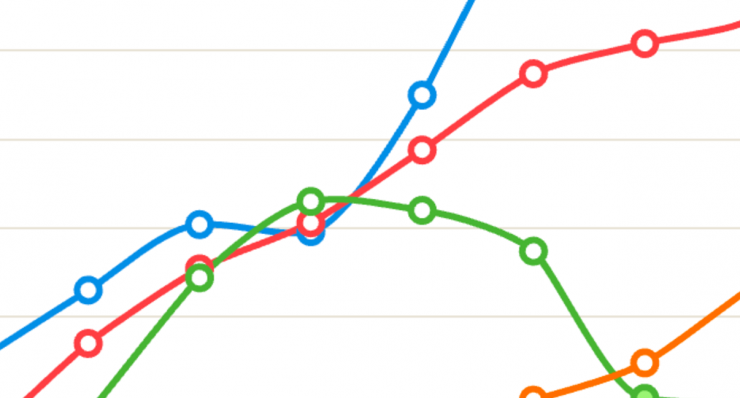
\includegraphics[width=\textwidth]{graph_a}
	\caption{$y=x$}
	\label{fig: y equals x}
	\end{subfigure}
	\caption{Tres figures}
	\label{fig:three_graphs}
\end{figure}
Lorem ipsum dolor sit amet, consectetur adipiscing elit. Integer bibendum arcu id scelerisque luctus. Morbi bibendum quam nisi, sed congue eros feugiat a. Cras sed sapien facilisis, vehicula lectus quis, efficitur diam. Etiam volutpat dui ut ligula hendrerit gravida. Etiam imperdiet risus consequat ullamcorper lacinia. Aenean at lorem et mauris tempor maximus. Suspendisse pulvinar sapien ante, nec pretium enim ultrices eget. Donec tristique congue aliquam. Sed pulvinar, quam quis lobortis scelerisque, nunc velit blandit orci, nec gravida nibh eros eu augue. Curabitur cursus sapien lorem, non sollicitudin odio lobortis quis. Sed fermentum, libero semper dapibus tincidunt, enim odio vestibulum orci, ac ultricies nisi velit in nisl. Phasellus id interdum massa. Duis feugiat convallis leo eget elementum.
\paragraph{Nulla et congue massa. Phasellus purus quam, tincidunt in feugiat sit amet, tincidunt ut enim. Quisque semper convallis lorem, quis vehicula est euismod nec.}
\paragraph{Nam interdum ipsum dolor, ut fringilla risus ullamcorper sit amet. Mauris condimentum dui eget neque ultrices, vitae posuere ipsum feugiat. Ut sed dignissim mi. Mauris enim justo, ultrices ut ullamcorper ac, facilisis in est. Pellentesque scelerisque ultrices purus maximus fringilla. Nunc vel sem sit amet dui cursus ultricies. Curabitur commodo rhoncus vehicula.}
asdfjksdfjsjfsjfkj\\
\newline
sdfksjkfsjdf
%
Per inserir una taula podem fer servir \verb|taula| i \verb|tabular|:
%
\begin{table}[h]
\centering
\begin{tabular}{l | l | l}
A & B & C \\
\hline
1 & 2 & 3 \\
4 & 5 & 6
\end{tabular}
\caption{Taula bàsica}
\label{tab:abc}
\end{table}
%
%
També podem inserir múltiples taules com a continuació. Si demanem massa amplada les taules poden saltar de línia. \verb|taula| i \verb|tabular|:
%
\begin{table}[h]
	\begin{subtable}[h]{0.45\textwidth}
		\centering
		\begin{tabular}{l | l | l}
		A & B & C \\
		\hline
		1 & 2 & 3 \\
		4 & 5 & 6
		\end{tabular}
		\caption{Taula}
		\label{tab:abc}
	\end{subtable}
	\hfill
		\begin{subtable}[h]{0.45\textwidth}
		\centering
		\begin{tabular}{l | l | l}
		A & B & C \\
		\hline
		1 & 2 & 3 \\
		4 & 5 & 6
		\end{tabular}
		\caption{Taula}
		\label{tab:abc}
	\end{subtable}
	\hfill
		\begin{subtable}[h]{0.45\textwidth}
		\centering
		\begin{tabular}{l | l | l}
		A & B & C \\
		\hline
		1 & 2 & 3 \\
		4 & 5 & 6
		\end{tabular}
		\caption{Taula}
		\label{tab:abc}
	\end{subtable} 
	\caption{Tres taules}
	\label{tab:temps}
\end{table}
%
%
%
Algunes taules més:
%https://www.overleaf.com/learn/latex/Tables
%
\begin{center}
\begin{tabular}{ c c c }
 cell1 & cell2 & cell3 \\ 
 cell4 & cell5 & cell6 \\  
 cell7 & cell8 & cell9    
\end{tabular}
\end{center}
%
\begin{center}
\begin{tabular}{ |c|c|c| } 
 \hline
 cell1 & cell2 & cell3 \\ 
 cell4 & cell5 & cell6 \\ 
 cell7 & cell8 & cell9 \\ 
 \hline
\end{tabular}
\end{center}

\begin{center}
 \begin{tabular}{||c c c c||} 
 \hline
 [0.5ex]  Col1 & Col2 & Col2 & Col3 \\ [0.5ex] 
 \hline\hline [0.5ex] 
 1 & 6 & 87837 & 787 \\ [0.5ex] 
 \hline [0.5ex] 
 2 & 7 & 78 & 5415 \\[0.5ex] 
 \hline
 3 & 545 & 778 & 7507 \\[0.5ex] 
 \hline
 4 & 545 & 18744 & 7560 \\[0.5ex] 
 \hline
 5 & 88 & 788 & 6344 \\ [0.5ex]  
 \hline
\end{tabular}
\end{center}

{\setlength{\extrarowheight}{3pt}%

\begin{center}
 \begin{tabular}{c | c c c} 
 \hline
 \multicolumn{4}{|c|}{Country List} \\
 \hline \hline
 Col1 & Col2 & Col2 & Col3 \\
 \hline
 1 & 6 & 87837 & 787 \\
 2 & 7 & 78 & 5415 \\ 
 3 & 545 & 778 & 7507 \\ 
 4 & 545 & 18744 & 7560 \\
 5 & 88 & 788 & 6344 \\
\end{tabular}
\end{center}

\begin{table}[h!]
\centering
 \begin{tabular}{c | c c c} 
 Col1 & Col2 & Col2 & Col3 \\
 \hline
 1 & 6 & 87837 & 787 \\
 \rowcolor[HTML]{b2f2ff}2 & 7 & 78 & 5415 \\ 
 3 & 545 & 778 & 7507 \\ 
 \rowcolor[HTML]{b2f2ff}4 & 545 & 18744 & 7560 \\
 5 & 88 & 788 & 6344 \\
\end{tabular}
\caption{Taula que vull fer servir per defecte}
\label{table:1}
\end{table}
%
\begin{tabular}{ |p{3cm}||p{3cm}|p{3cm}|p{3cm}|  }
 \hline
 \multicolumn{4}{|c|}{Country List} \\
 \hline
 Country Name     or Area Name& ISO ALPHA 2 Code &ISO ALPHA 3 Code&ISO numeric Code\\
 \hline
 Afghanistan   & AF    &AFG&   004\\
 Aland Islands&   AX  & ALA   &248\\
 Albania &AL & ALB&  008\\
 Algeria    &DZ & DZA&  012\\
 American Samoa&   AS  & ASM&016\\
 Andorra& AD  & AND   &020\\
 Angola& AO  & AGO&024\\
 \hline
\end{tabular}
%
\\
\newline
També podríem inserir una taula amb \textbf{tabularx} enlloc de \textbf{tabular}.\\
adfsf \\
%
%
\newline
%
\begin{table}[h!]
\centering
 \begin{tabular}{||c c c c||} 
 \hline
 Col1 & Col2 & Col2 & Col3 \\ [0.5ex] 
 \hline\hline
 1 & 6 & 87837 & 787 \\ 
 2 & 7 & 78 & 5415 \\
 3 & 545 & 778 & 7507 \\
 4 & 545 & 18744 & 7560 \\
 5 & 88 & 788 & 6344 \\ [1ex] 
 \hline
 \end{tabular}
\end{table}
%
\newline
The table \ref{table:1} is an example of referenced \LaTeX elements.
 %
\begin{table}[h!]
\centering
\begin{tabular}{||c c c c||} 
 \hline
 Col1 & Col2 & Col2 & Col3 \\ [0.5ex] 
 \hline\hline
 \rowcolor{gray} 1 & 6 & 87837 & 787 \\ 
 2 & 7 & 78 & \cellcolor[HTML]{AA0044} 5415 \\
 \rowcolor{gray} 3 & 545 & 778 & 7507 \\
 4 & 545 & 18744 & 7560 \\
 \rowcolor{gray} 5 & 88 & 788 & 6344 \\ [1ex] 
 \hline
\end{tabular}
\caption{Table to test captions and labels}
\label{table:2}
\end{table}




\subsection{Títol de la subsecció}
Lorem ipsum dolor sit amet, consectetur adipiscing elit. Integer bibendum arcu id scelerisque luctus. Morbi bibendum quam nisi, sed congue eros feugiat a. Cras sed sapien facilisis, vehicula lectus quis, efficitur diam. Etiam volutpat dui ut ligula hendrerit gravida. Etiam imperdiet risus consequat ullamcorper lacinia. Aenean at lorem et mauris tempor maximus. Suspendisse pulvinar sapien ante, nec pretium enim ultrices eget. Donec tristique congue aliquam. Sed pulvinar, quam quis lobortis scelerisque, nunc velit blandit orci, nec gravida nibh eros eu augue. Curabitur cursus sapien lorem, non sollicitudin odio lobortis quis. Sed fermentum, libero semper dapibus tincidunt, enim odio vestibulum orci, ac ultricies nisi velit in nisl. Phasellus id interdum massa. Duis feugiat convallis leo eget elementum.\\
\newline
Vivamus faucibus malesuada dolor, at euismod risus eleifend lobortis. In facilisis efficitur metus, eu commodo velit convallis eu. Pellentesque facilisis tincidunt nulla eget posuere. Nullam rutrum aliquam viverra. Maecenas ullamcorper nibh libero, sed venenatis orci ornare quis. Nulla facilisi. Morbi nisl tortor, cursus sit amet dignissim iaculis, aliquet ac quam. Nulla leo mi, condimentum quis nisl eu, pellentesque tincidunt metus. Donec lectus arcu, consequat a eleifend nec, venenatis rutrum dui. Quisque efficitur elit vel fermentum pharetra.\\
\newline
Nam nec tempus nibh. Nullam in orci eget ex suscipit porta. In nulla felis, hendrerit in lacinia consectetur, viverra in neque. Praesent volutpat turpis sed eros accumsan, eget luctus nulla porta. Curabitur sit amet auctor odio. Duis tincidunt lacus sed justo venenatis sodales. Class aptent taciti sociosqu ad litora torquent per conubia nostra, per inceptos himenaeos. Sed porta turpis quis cursus mollis. Quisque ipsum leo, gravida sit amet tellus ut, gravida rutrum leo. Proin vestibulum bibendum ligula a aliquam. Vivamus sit amet magna at justo tempor efficitur ut nec enim. Nulla semper erat vel nisi sollicitudin, ut auctor eros tempus. Aliquam molestie erat a justo molestie, vitae porttitor nisi blandit. Aenean sollicitudin ac erat scelerisque finibus. Nullam dignissim dictum aliquam. Phasellus dapibus malesuada ex ut placerat.
